\documentclass[10pt,a4paper]{article}
\usepackage[utf8]{inputenc}
\usepackage[spanish]{babel}
\usepackage{amsmath}
\usepackage{amsfonts}
\usepackage{amssymb}
\usepackage{makeidx}
\usepackage{graphicx}
\usepackage{lmodern}

\usepackage[left=2cm,right=2cm,top=3cm,bottom=2cm]{geometry}
\author{Daniel Vázquez Lago}
\title{Circuitos de Corriente Continua}
\begin{document}
\maketitle
\newpage
\tableofcontents
\newpage
\section{Circuito de Corriente Continua}


\subsection{Objetivos} 
Los principales objetivos de esta práctica serán: \begin{itemize}
\item Comprobar experimentalmente la Ley de Ohm y de las leyes básicas de asociación de resistencias.
\item La demostración de que el alumnado posee los conocimientos necesarios para hacer un riguroso y correcto tratamiento de los datos mediante el uso de la propagación de incertidumbres, el ajuste lineal (usando el método de mínimos cuadrados) y el correcta expresión de los mismos. Para ello contaremos con numerosas gráficas, tablas de datos y ecuaciones que nos permitirán explicar detalladamente el proceso de obtención de los resultados. 
\item El correcto uso del polímetro y aplicación del código de colores para las resistencias.
\end{itemize}
\subsection{Análisis de datos:  Medida de resistencias}

\begin{figure}[htb] %Figura de resistencias
\centering
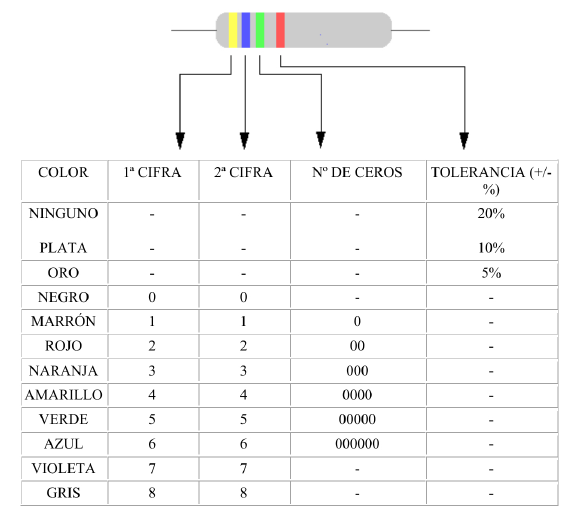
\includegraphics[width=12cm, height=10cm]{Resistencias}
\caption{Código de colores para las resistencias}
\label{fig: Resistencias}
\end{figure}

Como podemos observar tenemos una tabla de resistencias, que asocia los distintos colores que tiene una resistencia con su valor, calculado por el fabricante, con su tolerancia, que nos da un margen de los posibles valores de la resistencia, es decir, su incertidumbre.

\newpage

\begin{table}[t] %Tabla de resistencias de fabricante
\begin{center}
\begin{tabular}{| c | c | c | c |}
\hline
Resistencia & Valor nominal ($\Omega$) & Tolerancia (\%) & $R \pm s(R) \ (\Omega)$ \\ \hline
$R_1$ & $220000 $ &  5  & $220000 \pm 11000$\\
$R_2$ & $390000 $ &  5  & $390000 \pm 19500$ \\ \hline
\end{tabular}
\caption{Valor de las resistencias e incertidumbres según fabricante}
\label{tab:Resistencias fabricante}
\end{center}
\end{table}

\begin{table} %Tabla resistencias experimentalmente


\begin{center}
\begin{tabular}{| c | c | c | c |}
\hline
Resistencia & Lectura ($\Omega$) & Resolución ($\Omega$) & $R \pm s(R) \ (\Omega)$ \\ \hline
$R_1$ & $217 \cdot 10^3 $ & $10^3$  & $22 \cdot 10^3 \pm 10^3$\\
$R_2$ & $397 \cdot 10^3 $ & $10^3$  & $39 \cdot 10^3 \pm 10^3$ \\ \hline
\end{tabular}
\caption{Valor de las resistencias e incertidumbres experimentalmente}
\label{tab:Resistencias experimentalmente}
\end{center}
\end{table}
En la tabla \ref{tab:Resistencias fabricante} tenemos las resistencias que nos da el fabricante, en función de los colores de la resistencia y de sus valores asociados en la figura \ref{fig: Resistencias}. En la tabla \ref{tab:Resistencias experimentalmente} tenemos los valores de las resistencias calculadas experimentalmente mediante un polímetro. \\

Para calcular estos valores experimentales lo que hacemos es coger un polímetro con la parte de medir resistencias seleccionada, y poner los dos terminales en los extremos de las resistencias. \\

El motivo principal por el que hacemos dos cálculos de los valores de las resistencias es para comprobar si estas resistencias están realmente en los margenes de error que nos da el fabricante, y porque nos da una mayor exactitud para posteriores cálculos que realizaremos.
Como podemos observar ambas resistencias están dentro de los márgenes, ya que según el fabricante la resistencia uno debería estar en el rango $(209000,\ 231000)$ en el que claramente 217000 está; y la resistencia 2, con valor de 397000, está en el rango (370500, 4095000).\\

De esta forma cumplimos el tercer objetivo de esta práctica, ya que hemos aplicado el código de colores para las resistencias y hecho un correcto uso del polímetro para calcular estos valores, aunque esta parte será mas notoria más adelante.
\subsection{Análisis de datos: Circuito Paralelo}

Como bien sabemos, un circuito en paralelo la tiene la siguiente forma: 

\begin{figure}[htb] %Figura de circuito en paralelo
\centering
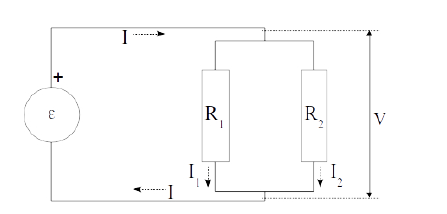
\includegraphics[width=12.5cm, height=5.5cm]{Paralelo}
\caption{Circuito en paralelo}
\label{fig: Resistencias}
\end{figure}

Ahora bien, como bien nos dice la ley de Ohm, este tipo de circuito equivale a un circuito con una única resistencia ($R_T$), que tiene el valor de:

\begin{equation}
 \dfrac{1}{R_T}=\sum_{k=1}^n \dfrac{1}{R_k}
 \label{Paralelo}
\end{equation}

Ahora bien, vamos a comprobar que esta ley fundamental se cumple mediante una medida directa, una estimación teórica y una estimación indirecta.
\subsubsection{Medida directa}
La medida directa no tiene mucho misterio. Al igual que antes, seleccionamos la parte de medir resistencias del polímetro, pero en este caso en vez de colocar los terminales en los extremos de las resistencias los colocaremos justo antes de los dos nodos. La siguiente tabla ilustrará cual es el valor y su incertidumbre:
\\
\begin{table}[h] %Medida directa

\begin{center}
\begin{tabular}{| c | c | c | c |}
\hline
Resistencia & Lectura ($\Omega$) & Resolución ($\Omega$) & $R \pm s(R) \ (\Omega)$ \\ \hline
$R_T$ & $1406 \cdot 10^2 $ & $10^2$  & $1406 \cdot 10^2 \pm 10^2$ \\ \hline
\end{tabular}
\caption{Valor de la resistencia equivalente mediante medida directa}

\label{tab:Paralelo 1}
\end{center}
\end{table}
\subsubsection{Estimación teórica}

La estimación teórica se hace usando la formula \ref{Paralelo}, y la incertidumbre se calcula mediante la propagación de incertidumbres, cuya fórmula es así:

\begin{equation}
s(y)=\sqrt{\sum_i (\dfrac{\partial y}{ \partial x_i})^2s^2(x_i)}
\label{Fórmula de propagación de incertidumbres}
\end{equation} 

En nuestro caso será:

\begin{equation}
s(R_T)=\sqrt{(\dfrac{\partial R_T}{ \partial R_1})^2s^2(R_1)+(\dfrac{\partial R_T}{ \partial R_2})^2s^2(R_2)}
\label{Propagación de incertidumbres estimación teórica}
\end{equation}

Y que las derivadas parciales son:

\begin{equation}
\dfrac{\partial R_T}{ \partial R_1}=\dfrac{\partial (\dfrac{R_1 \cdot R_2}{R_1 + R_2})}{\partial R_1}=\dfrac{R_2(R_1+R_2)-R_1 \cdot R_2}{(R_1+R_2)^2} = \dfrac{R_2^2}{(R_2+R_1)^2}
\end{equation}
\begin{equation}
\dfrac{\partial R_T}{ \partial R_2}=\dfrac{\partial (\dfrac{R_1 \cdot R_2}{R_1 + R_2})}{\partial R_2}=\dfrac{R_1(R_1+R_2)-R_1 \cdot R_2}{(R_1+R_2)^2} = \dfrac{R_1^2}{(R_2+R_1)^2}
\end{equation}

Ahora usando las incertidumbres y valores de la medida experimental de resistencias (tabla \ref{tab:Resistencias experimentalmente}), ya que son las más exactas, y tenemos los siguientes valores:

\begin{table}[h] %Tabla de parametros para la estimación teórica
\begin{center}
\begin{tabular}{| c | c | c | c | c |}
\hline

$R_i$ & Valor nominal ($\Omega$) & Incertidumbre ($\Omega$) & $R_i^2$ & $s(R_i)^2$ \\ \hline
$R_1$ & $217 \cdot 10^3$ & $10^3$ & $4.71 \cdot 10^{10}$ & 1000000 \\
$R_2$ & $397\cdot 10^3$ & $10^3$ & $1.58 \cdot 10^{11}$  & 1000000 \\ 
$R_1+R_2$ & $614\cdot 10^3$ & - & $3.77 \cdot 10^{11} $ & -\\ \hline
\end{tabular}
\caption{Valor de los diferentes parámetros que vamos a usar para calcular $R_T$ }
\end{center}
\end{table}

Una vez tenemos estos datos, podemos aplicar la fórmula \ref{Paralelo} y \ref{Propagación de incertidumbres estimación teórica} para calcular $R_T$ y su incertidumbre:
$$ \dfrac{1}{R_T}=\dfrac{1}{R_1}+\dfrac{1}{R_2} \Longrightarrow R_T=\dfrac{R_1 \cdot R_2}{R_1+R_2}=\dfrac{217 \cdot 10^3 \cdot 397\cdot 10^3}{397\cdot 10^3 + 217 \cdot 10^3}=140310 \cdot 10^1\ \Omega $$
$$ s(R_T)=\sqrt{10^6 \cdot \dfrac{(0,471+1,58)\cdot10^{11}}{3,77 \cdot 10^{11}}} =74 \cdot 10^1 $$
En el caso de la incertidumbre cogemos 2 cifras significativas porque al realizar cálculos mediante propagación de incertidumbres es la regla que usamos. En el caso de que nos dieran otras unidades posteriormente simplemente realizamos la aproximación. Una vez tenemos estos datos vamos a construir una tabla, que aunque bien sencilla, nos permitirá reflejar mejor los datos y compararlos posteriormente:


\begin{table}[h] %Tabla de parametros para la estimación teórica
\begin{center}
\begin{tabular}{| c | c | c | c | }
\hline

Resistencia & Valor nominal ($\Omega$) & Incertidumbre ($\Omega$) & $R_T \pm s(R_T)$\\ \hline
$R_T$ & $14031 \cdot 10^1 $ & $74 \cdot 10^1 $ & $14031 \cdot 10^1 \pm 74 \cdot 10^1$ \\ \hline
\end{tabular}
\caption{ Valor de las resistencia equivalente y su incertidumbre teórica}
\end{center}
\end{table}

\subsubsection{Estimación indirecta}
Como bien sabemos, la ley de Ohm nos dice que el voltaje total del sistema es igual a la intensidad por la resistencia:
\begin{equation} \label{Ley de Ohm}
V=I \cdot R
\end{equation}

Entonces es posible calcular la resistencia de un sistema sabiendo el voltaje y la intensidad que circula por el mismo. Debido a las características de la fórmula, si representamos voltaje frente a la intensidad, la pendiente de la recta será entonces el valor de la resistencia. Entonces tomando varias medidas del voltaje y la intensidad, y haciendo la representación tendremos una estimación indirecta del valor de la resistencia. Para calcular la incertidumbre, los valores de la pendiente... usaremos el método de mínimos cuadrados, haciendo una regresión lineal simple mediante el lenguaje python. \\

En primer lugar mostraremos los valores calculados experimentalmente, y que mas tarde usaremos:
\begin{table}[h] %Tabla de parametros para la estimación teórica
\begin{center}
\begin{tabular}{| c | c | c | c | c | c | c | c |}
\hline
Medida & $V \ (V)$ & s(V) & $I_1 $ (A) & $I_2 (A)$ & $I_1 + I_2 \ (A)$ & $ I \ (A)$ & s($I$) \\ \hline
1 & 1,0 & 0,1 & $5,0 \cdot 10^{-6}$ & $2,7 \cdot 10^{-6}$ & $ 7,7 \cdot 10^{-6}$ & $7,5 \cdot 10^{-6} $
& $0,1\cdot 10^{-6}$\\
2 & 2,0 & 0,1 & $9,4 \cdot 10^{-6}$ & $5,2 \cdot 10^{-6}$ & $ 14,6\cdot 10^{-6}$ & $ 14,7 \cdot 10^{-6} $ & 0$,1\cdot 10^{-6}$\\
3 & 3,0 & 0,1 & $14,1 \cdot 10^{-6}$ & $7,6 \cdot 10^{-6}$ & $ 21,7 \cdot 10^{-6}$ & $21,7 \cdot 10^{-6}$ & $0,1 \cdot 10^{-6}$\\
4 & 4,0 & 0,1 & $18,5 \cdot 10^{-6}$ & $10,3 \cdot 10^{-6}$ & $ 28,8 \cdot 10^{-6}$ & $28,9\cdot 10^{-6}$ & $0,1\cdot 10^{-6}$\\
5 & 5,0 & 0,1 & $23,2 \cdot 10^{-6}$ & $12,8 \cdot 10^{-6}$ & $ 36,0 \cdot 10^{-6}$ & $35,9\cdot 10^{-6}$ & $0,1\cdot 10^{-6}$\\
6 & 6,0 & 0,1 & $27,8 \cdot 10^{-6}$ & $15,3 \cdot 10^{-6}$ & $ 43,1 \cdot 10^{-6}$ & $43,2\cdot 10^{-6}$ & $0,1\cdot 10^{-6}$\\
7 & 7,0 & 0,1 & $32,3 \cdot 10^{-6}$ & $17,8 \cdot 10^{-6}$ & $ 50,1 \cdot 10^{-6}$ & $50,5\cdot 10^{-6}$ & $0,1\cdot 10^{-6}$\\
8 & 8,0 & 0,1 & $37,4 \cdot 10^{-6}$ & $20,4 \cdot 10^{-6}$ & $ 57,8 \cdot 10^{-6} $ & $57,5\cdot 10^{-6}$ & $0,1\cdot 10^{-6}$\\
9 & 9,0 & 0,1 & $41,7 \cdot 10^{-6}$ & $22,9 \cdot 10^{-6}$ & $ 64,6 \cdot 10^{-6}$ & $65,5\cdot 10^{-6}$ & $0,1\cdot 10^{-6}$\\
10 & 10,0 & 0,1 & $46,4 \cdot 10^{-6}$ & $25,4\cdot 10^{-6}$ & $ 71,8 \cdot 10^{-6}$ & $77,0\cdot 10^{-6}$ & $0,1\cdot 10^{-6}$\\ \hline
\end{tabular}
\caption{ Valor de las resistencia equivalente y su incertidumbre teórica}
\end{center}
\end{table}
\begin{flushleft}
Como podemos ver, tomamos también datos en $I_1$ e $I_2$, ya que la ley de asociación de resistencias nos dice que:
\end{flushleft}
\begin{equation}
I = \sum_{k=1}^n I_k \label{Intensidades paralelo}
\end{equation}
Entonces las calculamos por comprobar que la intensidad total calculada está correctamente calculada, además que así demostramos una de las leyes de asociaciones de resistencias para los circuitos en paralelo: que la intensidad total es igual a la suma de las intensidades de cada resistencia (colocando n resistencias en paralelo partiendo del mismo nodo).\\

Como ya mencionamos previamente, vamos a hacer una regresión lineal. Para esto se ha de suponer que existe un parámetro $\beta$ que relaciona dos magnitudes dadas, x e y, de tal forma que:
\begin{equation}
y = \alpha + \beta x \label{Dependencia función lineal}
\end{equation}

En nuestro caso los valores de y serán los valores del voltaje (V) y los valores de x serán los de la intensidad total (I). Además, debido a los errores existentes en la toma de datos (precisión, aproximaciones...) jamás vamos a poder encontrar $\beta$, nos tendremos que conformar una mera  aproximación, que será b. La existencia de $\alpha$ (cuya aproximación será a) también nos incomoda, ya que en la fórmula no aparece ningún termino independiente. Sin embargo, realmente nosotros tenemos que asumir que no sabemos la fórmula, y que este parametro tenemos que calcularlo, aunque después veremos que tiende a 0, y que por lo tanto podemos despreciarlo y que se cumple la formula, pero eso aún no lo sabemos. Ahora bien trataremos de que estos valores sean lo mas próximos sus valores reales mediante un proceso que ya mencionamos anteriormente: el método de mínimos cuadrados.\\

Entonces tenemos que las desviaciones serán de:
\begin{equation}
y_i-bx_i - a\neq 0 \label{Valor de las desviaciones}
\end{equation}
Y que entonces la suma de los productos de los cuadrados de estas desviaciones por el peso estadístico en cada punto es la cantidad a minimizar. Para esto respecto a b y a, e igualamos a 0:
\begin{equation}
\mathcal{X}^2=\sum_{i=1}^n w_i[y_i-bx_i-a]^2
\end{equation}

En nuestro caso definimos peso estadístico como:
\begin{equation}
w_i=[s(y_i)]^{-2} \label{peso estadístico}
\end{equation}
Ya que la incertidumbre de y del orden de 5 veces mas grande que la de x (y cuando lo elevamos al cuadrado es del orden de 10), es decir, se puede despreciar. Además como la incertidumbre de los valores de y es constante (0,1) decimos que $w=(0,1)^{-2}=100$. Entonces tomando w como constante y derivando respecto b y a tendríamos que:
\begin{equation}\label{minimos cuadrados}
-2\sum_{i=1}^n [x_i(y_i - bx_i-a)] = 0  \ \ \ \ \ -2\sum_{i=1}^n (y_i-a-bx_i)
\end{equation}
Obteniendo directamente las siguientes fórmulas:
\begin{equation}
b=\dfrac{n(\Sigma_i x_i y_i)-(\Sigma_i y_i)(\Sigma x_i)}{n(\Sigma x_i^2) -(\Sigma_i x_i)^2} \label{valor de b}
\end{equation}
\begin{equation}
a=\dfrac{ (\Sigma_i y_i)(\Sigma_i x_i^2)- (\Sigma_i x_i)(\Sigma_i x_iy_i)}{n(\Sigma_i x_i^2)-(\Sigma_i x_i)}\label{valor de a}
\end{equation}
El valor del coeficiente de de regresión lineal: 
\begin{equation}
r = \dfrac{n (\Sigma_i x_i y_i) - (\Sigma_i x_i)(\Sigma_i y_i)}{\sqrt{[n(\Sigma_i x_i^2)-(\Sigma_i x_i)^2][n(\Sigma_i y_i^2)-(\Sigma_i y_i)^2]}}
\end{equation}
Las incertidumbres asociadas son:
\begin{equation}
s=\sqrt{\dfrac{\Sigma_i (y_i-a-bx_i)^2}{n-2}}
\label{incertidumbre s}
\end{equation}
\begin{equation}
s(b)=s \sqrt{\dfrac{n}{n(\Sigma_i x_i^2)-(\Sigma_i x_i)^2}} 
\label{incertidumbre de b}
\end{equation}
\begin{equation}
s(a)=s \sqrt{\dfrac{\Sigma_i x_i^2}{n(\Sigma_i x_i^2)-(\Sigma_i x_i)^2} }
\label{incertidumbre de a}
\end{equation}
Una vez tenemos dichas fórmulas, solo hay que realizar cálculos. Para esto crearemos las siguientes tablas, para así dejar claro de donde aparecen los datos (aunque no se represente es evidente que $n=10$):
\begin{table}[h] %Tabla de parametros para la estimación teórica
\begin{center}
\begin{tabular}{| c | c | c | c | c | c |}
\hline i & $V_i \ \  (y_i)$ & $I_i \ \ (x_i)$ & $V_i \cdot I_i \ \ (x_iy_i)$ & $I_i^2 \ \ (x_i)^2$ & $V_i 2 \ \ (y_i)^2$
  \\ \hline
1 & 1,0 & 7,50E-06 & 7,50E-06 & 5,63E-11 & 1,0
  \\ 
2 & 2,0 & 1,47E-05 & 2,94E-05 & 2,16E-10 & 4,0
  \\ 
3 & 3,0 & 2,17E-05 & 6,51E-05 & 4,71E-10 & 9,0
  \\ 
4 & 4,0 & 2,89E-05 & 1,16E-04 & 8,35E-10 & 16,0
  \\ 
5 & 5,0 & 3,59E-05 & 1,80E-04 & 1,29E-09 & 25,0
  \\ 
6 & 6,0 & 4,32E-05 & 2,59E-04 & 1,87E-09 & 36,0
  \\ 
7 & 7,0 & 5,05E-05 & 3,54E-04 & 2,55E-09 & 49,0
  \\ 
8 & 8,0 & 5,75E-05 & 4,60E-04 & 3,31E-09 & 64,0
  \\ 
9 & 9,0 & 6,45E-05 & 5,81E-04 & 4,16E-09 & 81,0
  \\ 
10 & 10,0 & 7,20E-05 & 7,20E-04 & 5,18E-09 & 100,0
  \\  \hline
$\Sigma_i$ & 55,0 & 3,96E-04 & 2,77E-03 & 1,99E-08 & 3025,0  \\ \hline
 
\end{tabular}
\caption{Valores necesarios para calcular b (R), a y el coeficiente de regresión lineal (r)}
\end{center}
\end{table} 

Substituyendo los datos anteriores en las ecuaciones \ref{valor de a} y \ref{valor de b} tendríamos que:$a = -4.17849656 \cdot 10^{-2}$ y $b=139802$. Probablemente hayamos colocado cifras significativas de más, pero hasta que no hayamos calculado la incertidumbre no sabremos realmente con cuantas hay que representar los números. Por lo tanto colocamos de más, aunque luego representemos dichos números con las cifras significativas correctas.
Ahora bien, para calcular s(b) y s(a) hacen falta obtener un dato más, representado en la tabla 8. \\


\begin{table}[h] %Tabla de parametros estimación indirecta
\begin{center}
\begin{tabular}{| c | c | c |  }
\hline

i & $y_i -a -bx_i$ & $(y_i -a -bx_i)^2$ 
  \\ \hline
1 & -0,0067 & 0,000045
  \\ 
2 & -0,0133 & 0,000177 
  \\ 
3 & 0,0081 & 0,000065  
  \\ 
4 & 0,0015 & 0,000002  
  \\ 
5 & 0,0229 & 0,000523  
  \\ 
6 & 0,0023 & 0,000005  
  \\ 
7 & -0,0183 & 0,000333 
  \\ 
8 & 0,0031 & 0,000010  
  \\ 
9 & 0,0245 & 0,000600  
  \\ 
  10 & -0,0240 & 0,000577 
  \\ \hline
$\Sigma_i$ & $-4,66 \cdot 10^{-14}$ & 0,002338 \\  \hline
\end{tabular}

\label{tab: medida indirecta incertidumbres valores}
\caption{ Valor de las resistencia equivalente y su incertidumbre mediante la medida indirecta}
\end{center}
\end{table}

\begin{table}[h!]
\begin{center}
\begin{tabular}{| c | c | c | c | c |} \hline
b & s(b) & a & s(a) & r \\ \hline
$13980 \cdot 10^1 $& $26 \cdot 10^1$  & -0,042 & 0,012 & 0,99998 \\ \hline
\end{tabular}
\caption{Valores finales de la propagación de incertidumbres}
\end{center}
\end{table}


\begin{table}[h!] %Tabla de parametros estimación indirecta
\begin{center}
\begin{tabular}{| c | c | c | c | }
\hline

Resistencia & Valor nominal ($\Omega$) & Incertidumbre ($\Omega$) & $R_T \pm s(R_T)$\\ \hline
$R_T$ & $13980 \cdot 10^1 $ & $26 \cdot 10^1 $ & $13980 \cdot 10^1 \pm 26 \cdot 10^1 $ \\ \hline
\end{tabular}
\caption{ Valor de las resistencia equivalente y su incertidumbre mediante la medida indirecta}
\end{center}
\end{table}



\begin{figure}[h!] %Figura de resistencias
\centering
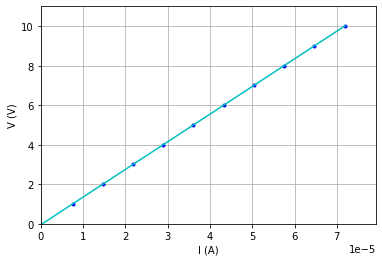
\includegraphics[width=10cm, height=7.5cm]{Plot}
\caption{Regresión lineal: Voltaje frente a Intensidad}
\label{fig: Resistencias}
\end{figure}
\newpage
Como podemos ver también hemos representado en la tabla 9 los valores de b, a (que ya en la siguiente subsección analizaremos), calculados con las anteriores ecuaciones. Además ahora si representamos a y b con las cifras significativas correctas. También calculamos r, que es una medida para saber cuan bien hecha está la regresión lineal. En nuestro caso nos da 0,99998 lo cual es muy buen indicativo: la regresión lineal esta muy bien hecha. 

\subsection{Comprobación ley de Ohm}
Como ya dijimos, uno de los objetivos de esta práctica es comprobar la ley de Ohm (y la ley de asociaciones de resistencias para el circuito paralelo). Para esto tomamos 3 formas de estudiar las resistencias, una de manera teórica, que es, en teoría, el valor que tiene que tener la resistencia equivalente del circuito. Entonces sabremos que se cumple dichas ecuaciones usadas si los valores que obtenemos de manera experimental están próximos a el valor teórico (dicho de otra forma, que están en el rango de su incertidumbre). El primer método experimental fue una medida directa, que esta evidentemente en el rango de incertidumbre. El segundo método experimental fue una medida indirecta, es decir, mediante la ley de Ohm (ecuación \ref{Ley de Ohm}), sabiendo la intensidad y voltaje total del circuito, calcular la resistencia total. Como se puede ver en la ley de Ohm, R es una constante que esta multiplicando a I. Es decir, si representamos V frente a I nos aparecerá una recta que en teoría pasa por el origen y cuya pendiente será la propia R. En esta misma relación se basa esta medida: calculamos la intensidad y voltaje del circuito, y tratamos de crear una recta que aproxime mejor los valores obtenidos mediante el método de mínimos cuadrados.  \\

De todos modos hay algo que no termina de encajar: si en teoría la relación I y V es directa, ¿Por qué a la hora de calcular dicha relación aparece un térmimo independiente a? La respuesta es bien sencilla: realmente no conocemos a ciencia cierta la ley de Ohm, ya que también estamos tratando de demostrarla, por lo tanto esta relación directa es \textit{desconocida} para nosotros. Sin embargo, se puede ver que este término independiente es irrisorio comparado con b. Podríamos casi considerarlo como consecuencia de la incertidumbre de tipo B, producto de la falta de precisión de los aparatos, condiciones ambientales no medibles... En resumen: se puede despreciar. De esta forma también comprobamos la propia ley de Ohm: ya que si la relación V e I se puede escribir como $V = bI$, y reescribimos b como R (cuadro 10) tenemos que $V = RI$. \\

De hecho, si escribimos la resistencia equivalente del circuito de las 3 formas que calculamos nos daremos cuenta de su similitud: 
$$ 140600 \footnote{Medida directa} \approx 140310 \footnote{Estimación teórica} \approx 139800  \footnote{Medida indirecta} $$
Como podemos ver si que están próximas. En conclusión: si que se cumple la ley de asociación de resistencias, y la ley de Ohm, cumpliendo parte del objetivo de esta práctica. No cabe olvidar que todo se ha realizado de manera rigurosa y exhaustiva, no cabiendo duda de la veracidad de dichas afirmaciones. 
\subsection{Conclusión}
Durante la práctica hemos usado tanto leyes básicas de la física y electricidad como las leyes de asociaciones de resistencias, ley de Ohm... así como las fórmulas de propagación de incertidumbres, recursos como \LaTeX, excel, python... \\

Con lo cual, si me preguntan cual es el significado de la práctica, yo diría que es probar que el alumnado tiene la capacidad de realzar un proyecto, que aunque no sea muy riguroso, ni tampoco complejo, de forma precisa, limpia y ordenada, comprobar su capacidad de expresarse correctamente usando un lenguaje científico, y si tiene que realizarlo en el día del mañana, estar preparado para abordarlo con unas nociones básicas. 
\section{Circuito de Corriente Alterna}
\subsection{Objetivos}
Los objetivos para esta práctica son:
\begin{itemize}
\item El uso de osciloscopio por parte del alumno, y que comprenda el funcionamiento de un circuito de corriente alterna y del condensador.
\item Obtener los parámetros característicos de la respuesta de un circuito RC, comprobar como funciona un condensador y mediante regresiones lineales representar gráficamente estos comportamientos. 
\item Específicamente en esta parte trataremos de calcular la frecuencia de corte, una frecuencia realmente importante en el mundo de la física e ingeniería, ya que es la frecuencia con la que la potencia se reduce un 50\% , sabiendo que $V_{mR} / V_{mC} = 1$, mediante un ajuste lineal; y como se comporta el desfase de la corriente alterna en función de la frecuencia y que para la frecuencia de corte el desfase tenemos un desfase de 45º.
\end{itemize}


\subsection{Análisis de datos }
\subsubsection{Frecuencia de corte}
En primer lugar tenemos que construir una tabla básica con los elementos que vamos a necesitar, obteniéndolos directamente del osciloscopio, que nos da directamente las amplitudes de los potenciales. En primer lugar configuramos el circuito así:


\begin{figure}[htb] %Osciloscopio 1
\centering
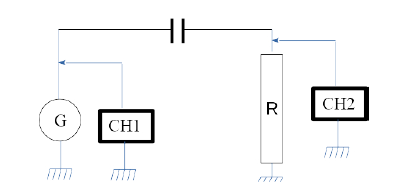
\includegraphics[width=6cm, height=3cm]{Osciloscopio 1}
\caption{Configuración del osciloscopio para calcular $V_{mR}$ }
\label{fig: Osciloscopio 1}
\end{figure}

De esta forma obtendríamos los diferencies valores de $V_{mR}$ en función de la frecuencia. La siguiente configuración sirve para calcular $V_{mC}$. Cabe destacar que aunque no salga la conexión a tierra del osciloscopio (CH1) esta justamente debajo de G (que es la fuente fem).

\begin{figure}[htb] %Osciloscopo 2
\centering
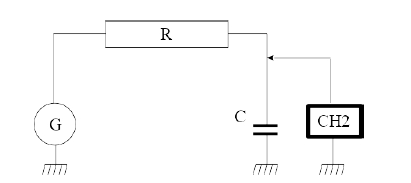
\includegraphics[width=6cm, height=3cm]{Osciloscopio 2}
\caption{Configuración del osciloscopio para calcular $V_{mC}$ }
\label{fig: Osciloscopio 2}
\end{figure}
Antes de continuar con la regresión lineal (que es lo que nos ataña) daremos cuenta de las incertidumbres de los elementos que vamos a usar. Teniendo en cuenta la ecuación 2 tenemos que: 
\begin{equation}
s(V_{mR}/V_{mC})=\sqrt{(-\dfrac{V_{mR}}{V_{mC}^2})^2 s^2(V_{mR}) + (\dfrac{1}{V_{mC}})^2s^2(V_{mR})}
\end{equation}
y sabiendo que las incertidumbres de tanto $V_{mr}$,$V_{mC}$ y $f$,  son las propias incertidumbres de los aparatos tenemos la incertidumbre de todo. Esto en realidad es bastante importante, ya que como se puede ver s(f) es despreciable frente a s($V_{mR} / V_{mC}$). Además para facilitar los cálculos, haremos que s($V_{mR} / V_{mC}$) sea constante, y la más alta de ellas (0,48), ya que hacerlo de otra forma llegaría a complicar mucho los cálculos, aunque sepamos que esto es incorrecto, o al menos no todo lo correcto que podría ser. \\


Ahora si, tendríamos los datos necesarios para realizar la regresión lineal, y calcular la frecuencia de corte a partir de esta, ya que sabemos teóricamente que el valor de $V_{mR}/V_{mC}=1$ para esta frecuencia particular. Sin embargo, antes de ello calcularemos la frecuencia de corte teórica, ya que si no, no podremos comprobar la veracidad de dichas formulas (que es parte del objetivo de la práctica). Además así podremos estimar lo cerca (o lejos) que están nuestro cálculo de dicho valor. Sabemos que la frecuencia de corte es un valor que cumple:

\begin{equation}
\label{Frecuencia de corte teoría}
f_c=\dfrac{1}{2 \pi R C}
\end{equation}

Y como $R=10 k\Omega$, $C=12 \cdot 10^{-9}$, tendríamos que $f_c=1326 Hz $, y calculando su incertidumbre tendríamos que s($f_c$)=133. Una  vez hecho esto, el siguiente paso es construir la regresión lineal. Para esto introducimos la tabla 12, con aquellos datos necesarios para calcular la regresión lineal. Debemos recordar que en esta regresión estamos calculando el cociente de los voltajes frente la frecuencia, por lo tanto $x_i$ serán los valores de la frecuencia, y $y_i$ el del cociente.. \\

Entonces la regresión lineal quedará como: $\dfrac{V_{mR}}{V_{mC}} = b \cdot f + a $, y si $\dfrac{V_{mR}}{V_{mC}} = 1$ tenemos que $f=\dfrac{1-a}{b}=1354$. Representando gráficamente los valores calculados experimentalmente en azul, y el valor donde $\dfrac{V_{mR}}{V_{mC}}=1$ con un punto negro.
Los valores con los que calculamos $f_c$ están en la tabla número 13, calculados con las ecuaciones anteriores (13, 14, 15, 17 y 18). \


Tal y como podemos observar la regresión lineal se cumple: prácticamente todos los puntos están en la línea, todos menos uno. Si quisiéramos mejorar la regresión lineal lo que podríamos hacer es repetir (o incluso de descartar) dicho valor, ya que se sobresale bastante de los datos anteriores. De todos modos el coeficiente de regresión lineal es muy bueno, (recordemos que cuanto mas se acerque a la unidad mejor) y en este caso es de 0,9996. Comparando el valor de $f_c$ calculado teóricamente y el recién calculado podemos ver que se acercan mucho, ya que $1326 \approx 1354$, aunque esto lo discutiremos profundamente mas adelante. \\

\begin{table} %Potenciales versus frecuencia
\begin{center}
\begin{tabular}{| c | c | c | c | c | c | c | c |} 
\hline$ f  \ (Hz) $ & $ s(f) (Hz) $ & $V_{mR} \ (V)$ & $ s(V_{mR}) (V)$  & $V_{mC} \ (V)$ & $ s(V_{mC}) (V) $ & $V_{mR} / V_{mC} $ & $ s(V_{mR} / V_{mC})$
  \\  \hline
100 & $10^{-6}$ & 1,52 & 0,02 & 20,0 & 0,20 & 0,0760 & 0,0039
  \\ 
200 & $10^{-6}$ & 3,02 & 0,02 & 19,8 & 0,20 & 0,1535 & 0,0079
  \\ 
300 & $10^{-6}$ & 4,44 & 0,02 & 19,6 & 0,20 & 0,227 & 0,012
  \\ 
400 & $10^{-6}$ & 5,80 & 0,02 & 19,2 & 0,20 & 0,302 & 0,016
  \\ 
500 & $10^{-6}$ & 7,04 & 0,02 & 18,8 & 0,20 & 0,374 & 0,020
  \\ 
600 & $10^{-6}$ & 8,30 & 0,02 & 18,3 & 0,20 & 0,454 & 0,025
  \\ 
700 & $10^{-6}$ & 9,4 & 0,20 & 17,7 & 0,20 & 0,531 & 0,031
  \\ 
800 & $10^{-6}$ & 10,4 & 0,20 & 17,2 & 0,20 & 0,605 & 0,036
  \\ 
900 & $10^{-6}$ & 11,2 & 0,20 & 16,7 & 0,20 & 0,671 & 0,041
  \\ 
1000 & $10^{-6}$ & 12,1 & 0,20 & 16,0 & 0,20 & 0,756 & 0,048
  \\ 
1300 & $10^{-6}$ & 14,0 & 0,20 & 14,4 & 0,20 & 0,972 & 0,069
  \\ 
1600 & $10^{-6}$ & 15,4 & 0,20 & 13,0 & 0,20 & 1,185 & 0,093
  \\ 
1900 & $10^{-6}$ & 16,4 & 0,20 & 11,6 & 0,20 & 1,414 & 0,124
  \\ 
2200 & $10^{-6}$ & 17,0 & 0,20 & 10,4 & 0,20 & 1,635 & 0,160
  \\ 
2500 & $10^{-6}$ & 17,6 & 0,20 & 9,5 & 0,20 & 1,853 & 0,199
  \\ 
2800 & $10^{-6}$ & 18,0 & 0,20 & 8,70 & 0,02 & 2,069 & 0,238
  \\ 
3100 & $10^{-6}$ & 18,5 & 0,20 & 8,50 & 0,02 & 2,176 & 0,256
  \\ 
3400 & $10^{-6}$ & 18,7 & 0,20 & 7,48 & 0,02 & 2,500 & 0,334
  \\ 
3700 & $10^{-6}$ & 18,9 & 0,20 & 7,00 & 0,02 & 2,700 & 0,386
  \\ 
4000 & $10^{-6}$ & 19,0 & 0,20 & 6,52 & 0,02 & 2,914 & 0,447
  \\ \hline
\end{tabular}
\label{tabla impedancia  capacitiva}
\caption{Potenciales vs frecuencia}
\end{center}
\end{table}

\begin{table} %Datos para la regresión lineal
\begin{center}
\begin{tabular}{| c | c | c | c | c | c | c | c |}
\hline

Medida (i) & $ x_i (f) $ & $ y_i (V_{mR} / V_{mC}) $ & $xi \cdot yi$ & $(xi ^ 2)$ & $(yi ^ 2)$ & $ \Sigma_i (y_i -a - bx_i) $ & $ \Sigma_i (y_i -a - bx_i)^2 $
  \\ \hline
1 & 100 & 0,076 & 7,6 & 10000 & 0,0058 & -0,015 & 0,00023
  \\ 
2 & 200 & 0,153 & 30,5 & 40000 & 0,0233 & -0,011 & 0,00013
  \\ 
3 & 300 & 0,227 & 68,0 & 90000 & 0,0513 & -0,010 & 0,000094
  \\ 
4 & 400 & 0,302 & 120,8 & 160000 & 0,0913 & -0,00659 & 0,000043
  \\ 
5 & 500 & 0,374 & 187,2 & 250000 & 0,1402 & -0,00667 & 0,000045
  \\ 
6 & 600 & 0,454 & 272,1 & 360000 & 0,2057 & -0,00005 & 0,0000000029
  \\ 
7 & 700 & 0,531 & 371,8 & 490000 & 0,2820 & 0,0050 & 0,000025
  \\ 
8 & 800 & 0,605 & 483,7 & 640000 & 0,3656 & 0,00611 & 0,000037
  \\ 
9 & 900 & 0,671 & 603,6 & 810000 & 0,4498 & -0,00034 & 0,000000
  \\ 
10 & 1000 & 0,756 & 756,3 & 1000000 & 0,5719 & 0,013 & 0,00016
  \\ 
11 & 1300 & 0,972 & 1263,9 & 1690000 & 0,9452 & 0,011 & 0,00013
  \\ 
12 & 1600 & 1,185 & 1895,4 & 2560000 & 1,4033 & 0,0064 & 0,000040
  \\ 
13 & 1900 & 1,414 & 2686,2 & 3610000 & 1,9988 & 0,018 & 0,00033
  \\ 
14 & 2200 & 1,635 & 3596,2 & 4840000 & 2,6720 & 0,022 & 0,00046
  \\ 
15 & 2500 & 1,853 & 4631,6 & 6250000 & 3,4322 & 0,022 & 0,00049
  \\ 
16 & 2800 & 2,069 & 5793,1 & 7840000 & 4,2806 & 0,021 & 0,00045
  \\ 
17 & 3100 & 2,176 & 6747,1 & 9610000 & 4,7370 & -0,089 & 0,00788
  \\ 
18 & 3400 & 2,500 & 8500,0 & 11560000 & 6,2500 & 0,017 & 0,00030
  \\ 
19 & 3700 & 2,700 & 9990,0 & 13690000 & 7,2900 & -0,000036 & 0,0000000013
  \\ 
20 & 4000 & 2,914 & 11656,44 & 16000000 & 8,4920 & -0,00332 & 0,000011
  \\ \hline
$\Sigma_1$  & 32000 & 23,565 & 59661,4 & 81500000 & 43,6881 & - & 0,011
  \\  \hline
\end{tabular}
\label{Desfases}
\caption{Datos para la regresión lineal}
\end{center}

\end{table}

\newpage 

\begin{table}[h] %Valores finales
\begin{center}
\begin{tabular}{|c|c|c|c|c|}
\hline
a & s(a) & b & s(b) & r 
  \\ \hline
0,01881 & 0,0090 & 0,00072466 & 0,0000045 & 0,9996 \\
\hline
\end{tabular}
\end{center}
\label{Datos de la regresión lineal}
\caption{Datos finales de la regresión lineal}
\end{table}

\begin{figure}[h!] %Figura de regresión lineal
\centering
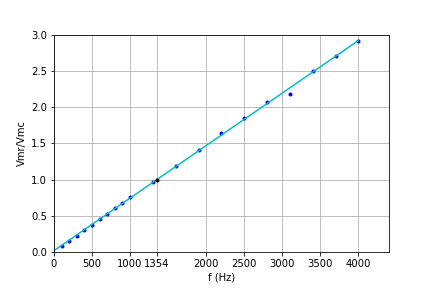
\includegraphics[width=12cm, height=9cm]{Plot1}
\caption{Regresión lineal: potenciales vs frecuencia}
\label{fig: Potenciales vs frecuencia}
\end{figure}



\subsubsection{Desfase entre señales}

Para calcular el desfase entre señales hay que configurar el osciloscopio en modo dual para visualizar las señales del generador ($V_G$) y de la resistencia ($V_R$). El desfase entre señales es la diferenia de fase que hay entre un máximo de la onda en el generador y la resistencia, lo que conlleva a que en un determinado instante uno tenga el máximo, y en otro instante la otra tenga su máximo. La diferencia de tiempo es la diferencia entre ambos tiempos. En función de cual sea nuestra señal de referencia, tendremos que esta diferencia ($\Delta t$) será positiva o negativa. En nuestro caso cogimos como referencia ($t_1$) el máximo de $V_R$, y $t_2$  el máximo de $V_G$. Esto lo que conllevo es que nuestra fase es negativa, pero realmente no cambia nada, ya que al  cambiar la referencia no cambiarían los datos, solo el signo. \\

Como hemos dicho, la fase depende de $\Delta t$, ya que si nos fijamos en la siguiente imagen: 
\begin{figure}[htb]
\center
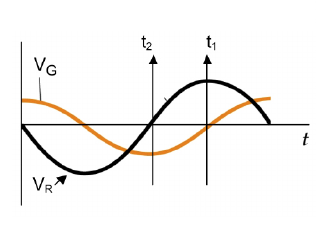
\includegraphics[width=6cm, height=4cm]{Desfase}
\label{Desfase}

\end{figure}

la diferencia de fase y esta diferencia del tiempo están directamente relacionados, de tal manera que:
\begin{equation}
\label{Desfase en grados}
\varphi = -2 \pi f \Delta t
\end{equation}

Esto nos permite obtener la siguiente tabla a partir de la diferencia del tiempo, y con sus incertidumbres, calculadas con la fórmula 2:
\begin{table}[h] %Desfases en función de la frecuencia


\begin{center}
\begin{tabular}{| c | c | c | c | c | c | c | c |}
\hline
$f(Hz)$ & $s(f) (Hz) $ & log $ f $ & $\varphi \ (rad) $ & $\varphi \ ($º) & $ s(\varphi$) (º) & $\Delta t \ (\nu seg) $ & $s(\Delta t)  (s) $ 
  \\ \hline
100 & $10^{-6}$ & 2 & 1,508 & 86,4 & 3,6 & 0,0024 & $10^{-4}$
  \\ 
200 & $10^{-6}$ & 2,30 & 1,407 & 80,6 & 0,072 & 0,001120 & $10^{-6}$
  \\ 
300 & $10^{-6}$ & 2,48 & 1,357 & 77,8 & 0,11 & 0,000720 & $10^{-6}$
  \\ 
400 & $10^{-6}$ & 2,60 & 1,257 & 72,0 & 0,14 & 0,000500 & $10^{-6}$
  \\ 
500 & $10^{-6}$ & 2,70 & 1,225 & 70,2 & 0,18 & 0,000390 & $10^{-6}$
  \\ 
600 & $10^{-6}$ & 2,78 & 1,206 & 69,1 & 0,22 & 0,000320 & $10^{-6}$
  \\ 
700 & $10^{-6}$ & 2,85 & 1,232 & 70,6 & 0,25 & 0,000280 & $10^{-6}$
  \\ 
800 & $10^{-6}$ & 2,90 & 1,056 & 60,5 & 0,29 & 0,000210 & $10^{-6}$
  \\ 
900 & $10^{-6}$ & 2,95 & 1,018 & 58,3 & 0,32 & 0,000180 & $10^{-6}$
  \\ 
1000 & $10^{-6}$ & 3,00 & 0,880 & 50,4 & 0,36 & 0,000140 & $10^{-6}$
  \\ 
1300 & $10^{-6}$ & 3,11 & 0,817 & 46,8 & 0,47 & 0,000100 & $10^{-6}$
  \\ 
1600 & $10^{-6}$ & 3,20 & 0,704 & 40,3 & 0,58 & 0,000070 & $10^{-6}$
  \\ 
1900 & $10^{-6}$ & 3,28 & 0,597 & 34,2 & 0,68 & 0,000050 & $10^{-6}$
  \\ 
2200 & $10^{-6}$ & 3,34 & 0,498 & 28,5 & 0,79 & 0,000036 & $10^{-6}$
  \\ 
2500 & $10^{-6}$ & 3,40 & 0,408 & 23,4 & 0,90 & 0,000026 & $10^{-6}$
  \\ 
2800 & $10^{-6}$ & 3,45 & 0,387 & 22,2 & 1,0 & 0,000022 & $10^{-6}$
  \\ 
3100 & $10^{-6}$ & 3,49 & 0,390 & 22,3 & 1,1 & 0,000020 & $10^{-6}$
  \\ 
3400 & $10^{-6}$ & 3,53 & 0,385 & 22,0 & 1,2 & 0,000018 & $10^{-6}$
  \\ 
3700 & $10^{-6}$ & 3,57 & 0,302 & 17,3 & 1,3 & 0,000013 & $10^{-6}$
  \\ 
4000 & $10^{-6}$ & 3,60 & 0,276 & 15,8 & 1,4 & 0,000011 & $10^{-6}$
  \\ \hline
\end{tabular}
\label{Desfases}¡
\caption{Desfases en función de la frecuencia}
\end{center}

\end{table}

\begin{figure}[h] %Figura de regresión lineal

\center
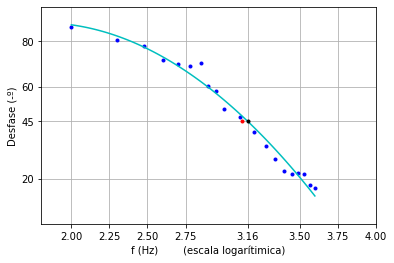
\includegraphics[width=12cm, height=9cm]{Plot2}
\caption{Desafase vs frecuencia}
\label{fig: Desfase vs frecuencia}
\end{figure}

La siguiente figura representa gráficamente los valores de la fase en grados sexagesimales en función de las diferentes frecuencias \footnote{En escala logarítimica}. La curva que podemos ver es una aproximación hecha por python con un polinomio de grado dos, de forma que se pueda observar la curva, ya que representarlo por una regresión lineal no solo sería una mala aproximación, si no que tampoco nos ayuda a ver como es la gráfica, ya que realmente es una curva, pero repito: no es mas que una aproximación, por lo tanto no es realista, ni mucho menos. Por esa misma razón la frecuencia equivalente a los 45 grados (en nuestro caso los -45º, aunque realmente la diferencia de fase no cambia) está bastante distorsionada . \\

De hecho, si calculamos $10^{3,26}$, que es el valor que nos da según dicha aproximación tenemos 1445 Hz, que aunque próximo, no es el valor calculado teóricamente, que sería el punto rojo (con frecuencia de 1326 Hz, en escala logarítmica $10^{3.12} Hz$). Como vemos no se distancian mucho realmente, y dicha diferencia se podría explicar perfectamente mediante la propagación de incertidumbre. \\

\subsection{Conclusiones}
Bien, una vez recopilados todos los datos y representadas las gráficas podemos discutir sobre el principal quid de esta parte de la práctica, que nos marcamos como objetivo: ¿Se cumple realmente que para la frecuencia de corte $V_{mR}/V_{mC}=1$ y que $\varphi = -45$º? \\

Como ya hemos adelantado antes, que para la frecuencia de corte  $V_{mR}/V_{mC}=1$ se cumple, ya que ambos datos son muy similares, teniendo en cuenta el número de medidas y la precisión de los aparatos (y que hay un dato que se sale por mucho de la medida) las cifras son muy similares:
$$ 1326 \approx 1354 $$ (y teniendo en cuenta que la incertidumbre teórica es de 133 todavía más).
Por lo tanto se puede afirmar con cierta seguridad que se cumple dicha regla.. \\

La segunda parte de la pregunta es mas difícil de afirmar, sobretodo por la no existencia de una regresión lineal, con lo cual la representación gráfica es mucho más inexacta, y sobretodo las conclusiones que podamos obtener de ella. Sin embargo, se puede ver como en la imagen \ref{fig: Desfase vs frecuencia} el punto rojo \footnote{Frecuencia de corte teórica} esta prácticamente  al lado del negro \footnote{Valor de la frecuencia de corte para los 45º aproximándonos por una parábola realizada por python}. Como antes no podemos afirmar que se cumple con total seguridad, ya que requeriría un estudio mas detallado (y más precisión), pero con dichos resultados podemos intuir la respuesta: que si se cumple. \\

Además, cumplimos el resto de los objetivos casi de manera indirecta, ya que para realizar estos gráficos e incertidumbres ya hace falta  poseer un mínimo conocimiento del osciloscopio, como funciona un condensador, y entender como es un circuito de corriente alterna. \\

A diferencia de la primera parte de la práctica, que se centraba más en como se propagaban las incertidumbres, los cálculos y como hacer un riguroso estudio experimental, esta parte se centra más en realmente aprender sobre un circuito de corriente alterna y condensadores, aunque no hay que ignorar que también perfeccionamos esta parte e incluso reforzamos los conocimientos las representaciones gráficas.
\end{document}
